\documentclass{article}
\usepackage[utf8]{inputenc}
\usepackage{listings}
\usepackage{graphicx}
\usepackage{xcolor}

\definecolor{codegreen}{rgb}{0,0.6,0}
\definecolor{codegray}{rgb}{0.5,0.5,0.5}
\definecolor{codepurple}{rgb}{0.58,0,0.82}
\definecolor{backcolour}{rgb}{0.95,0.95,0.92}

\lstdefinestyle{mystyle}{
    backgroundcolor=\color{backcolour},   
    commentstyle=\color{codegreen},
    keywordstyle=\color{magenta},
    numberstyle=\tiny\color{codegray},
    stringstyle=\color{codepurple},
    basicstyle=\ttfamily\footnotesize,
    breakatwhitespace=false,         
    breaklines=true,                 
    captionpos=b,                    
    keepspaces=true,                 
    numbers=left,                    
    numbersep=5pt,                  
    showspaces=false,                
    showstringspaces=false,
    showtabs=false,                  
    tabsize=2
    frame=single,
    float=H,
}

\lstset{style=mystyle}

\title{Linear Programming and Network Flows Final Report}
\author{Steven Glasford}
\date{15 May 2020}

\begin{document}

\maketitle
\begin{center}
    \textbf{All figures are attached to the bottom of this document and all of the python code for the parts of the project exist first within the their particular sections}
\end{center}
\section{Part 1}
\lstinputlisting[language=Python]{Part1.py}
For the code for part 1 please refer to figure above. This produces the output in figure \ref{fig:part1output}, which also produces the graph seen in figure \ref{fig:part1display}. \\
To answer the question poised in this part, we are able to conduct testing on this code by making calculations on the matrix distinct from those calculations provided in NetworkX, which is what is apparent at the end (lines 16, 17, and 18) of figure \ref{fig:part1output}.



\section{Part 2}
\lstinputlisting[language=Python]{Part2.py}
The code for this section can be found in figure above.
\\Part 2 required many different graphs to be outputted in particular degree centrality (figure \ref{fig:part2degree}), closeness centrality (figure \ref{fig:part2closeness}), betweenness centrality (figure \ref{fig:part2betweenness}), harmonic centrality (figure \ref{fig:part2harmonic}), eigenvector centrality (figure \ref{fig:part2eignenvector}), page rank (figure \ref{fig:part2pagerank}), and clustering (figure \ref{fig:part2clustering}). 
\\The output for this python code can be found in figure \ref{fig:part2output}.

\section{Part 3}
\lstinputlisting[language=Python]{Part3.py}

The code for this section can be found in figure above. There were several problems with the running of this code however, the only graph that was really able to run and display properly (as in display something that wasn't completely blackended by arcs to nodes as in figure \ref{fig:part3circular}), was the Spring layout drawing (figure \ref{fig:part3spring}).
\begin{itemize}
    \item \textbf{Circular}: too big and not much information (figure \ref{fig:part3circular})
    \item \textbf{Kamanda Kawai}: I could not run this graph in a reasonable amount of time, and system seemed to hang for hours.
    \item \textbf{Planar}: Our nodes are not planar so they cannot be represented in a plane.
    \item \textbf{Random}: Graph is too big, not much information is shown.
    \item \textbf{Spectral}: Took too long (several hours and produced nothing).
    \item \textbf{Spring}: The most interesting of the graphs, there is a level of separation in the graph that made it more interesting, however the user needs to zoom into the figure in order to actually see much information and it over all looks very chaotic. Figure \ref{fig:part3spring}.
    \item \textbf{Shell}: Looks very similar to the circular drawing in figure \ref{fig:part3circular}, which again doesn't show very much information.
\end{itemize}
\\In the end none of the graphs look very interesting or have too much information to extrapolate very much useful insight into the data, maybe Kamada Kawai is a good looking graph but it took too long to run on my machine and proved to be unsuccessful for me. The spring graph was a good looking graph, but its data is still bunched up to a point in which the data one can extrapolate from is limited.
\\
\\
\\
The next part of part 3 had us us a program called deepwalk, after installation I ran the statement in figure \ref{fig:part3deepwalk}. This produced a file that needed the first line removed, so instead of writing code to do that, I simply just edited the file and removed the first line in the file. Next,  I added the code starting from line 43 until the end of the file in figure for the code in part 3.
This resulted in a completely linear output as seen in figure \ref{fig:part3deepwalkgraph}.

\\
\\
\\
\section{End Remarks}
Thank you for being a wonderful professor, you have been one of my favorite professor this semester. Stay healthy.

\pagebreak


\begin{figure}
    \centering
    \lstinputlisting{part1.out}
    \caption{Part 1 output}
    \label{fig:part1output}
\end{figure}


\begin{figure}
  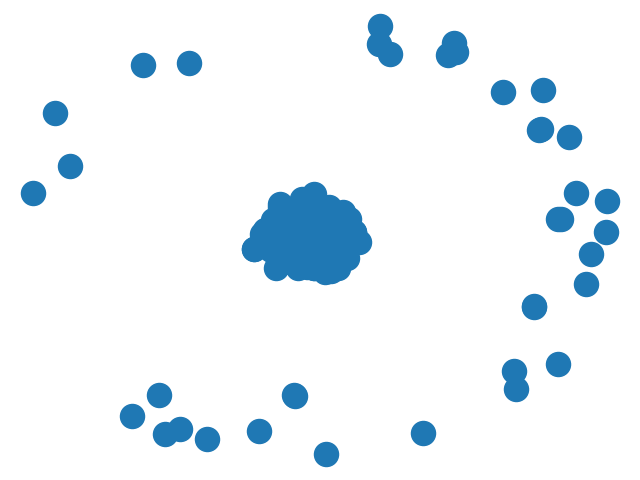
\includegraphics[width=\textwidth,height=\textheight,keepaspectratio]{protein_network.png}
  \caption{Network of Proteins for Homo Sapiens}
  \label{fig:part1display}
\end{figure}

\begin{figure}
    \centering
    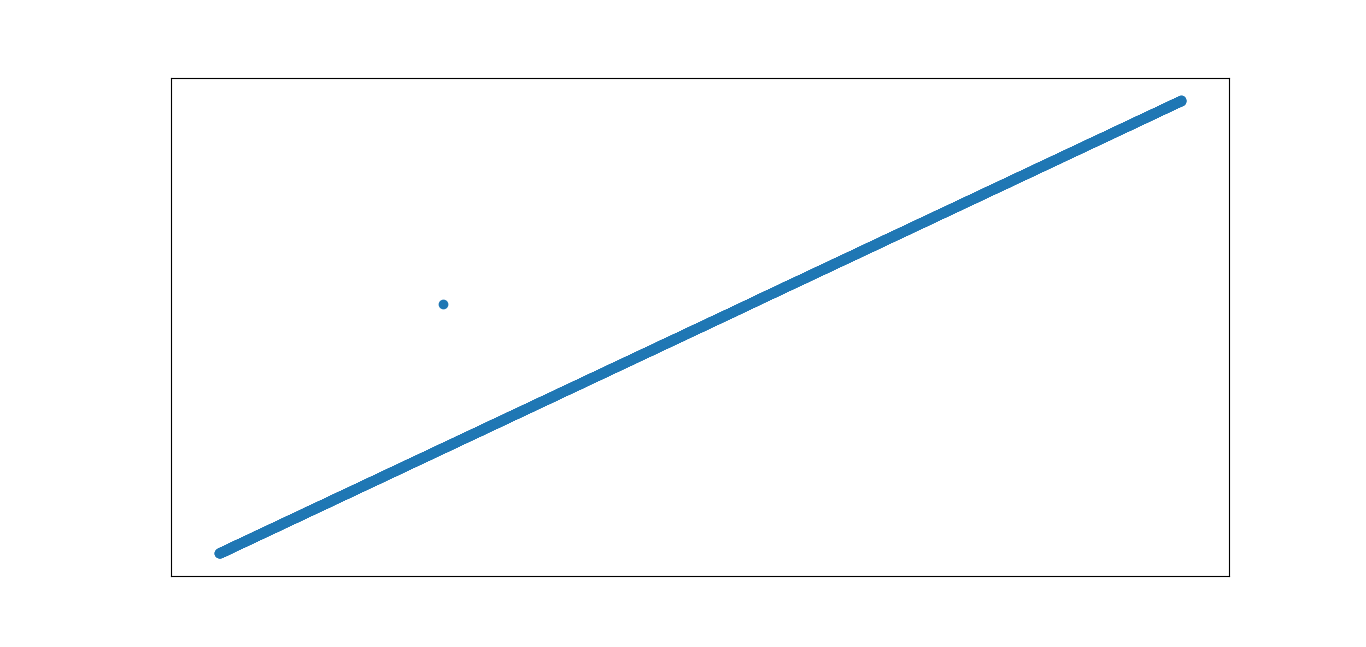
\includegraphics[width=\textwidth,height=\textheight,keepaspectratio]{deepwalk_graph.png}
    \caption{The graph produced by deep walk}
    \label{fig:part3deepwalkgraph}
\end{figure}



\begin{figure}
    \centering
    \lstinputlisting[width=\textwidth,height=\textheight,keepaspectratio]{deepwalkInput.txt}
    \caption{Command to run deepwalk on our dataset}
    \label{fig:part3deepwalk}
\end{figure}


\begin{figure}
    \centering
    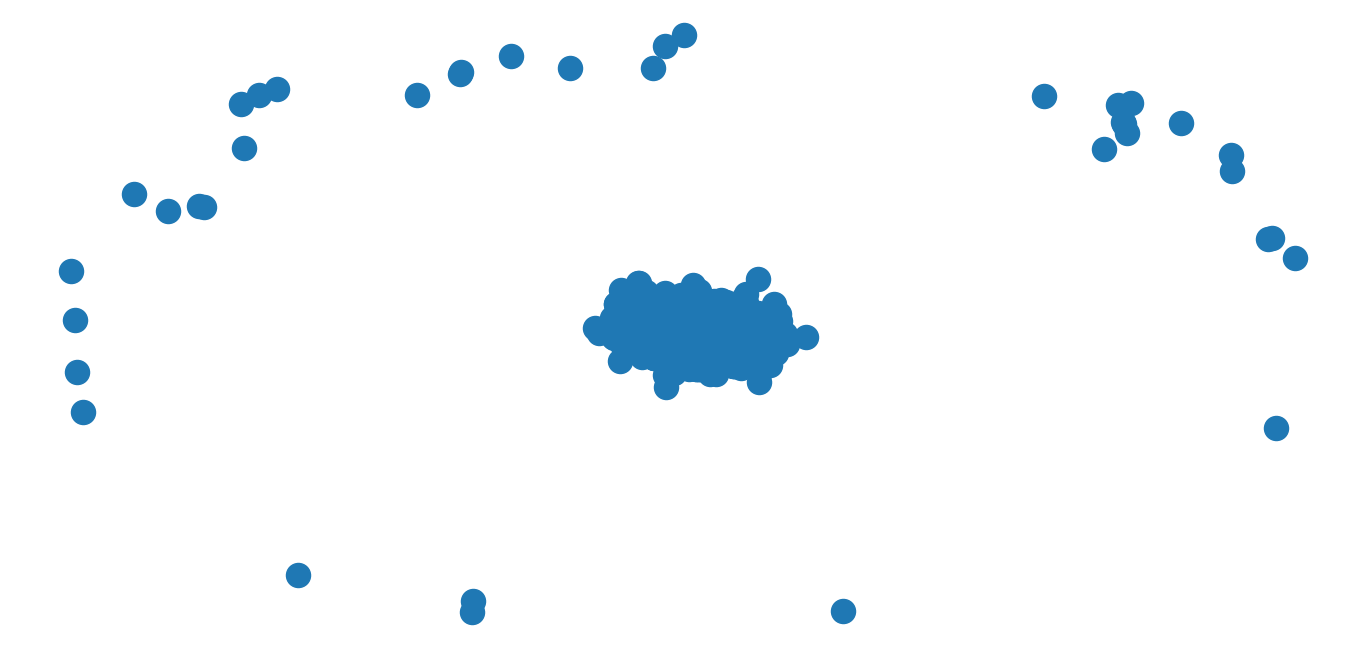
\includegraphics[width=\textwidth,height=\textheight,keepaspectratio]{spring_draw.png}
    \caption{Spring drawing for part 3}
    \label{fig:part3spring}
\end{figure}

% \begin{figure}[!htp]
%     \centering
%     \lstinputlisting[language=Python]{Part3.py}
%     \caption{Python code for Part 3}
%     \label{fig:part3code}
% \end{figure}

\begin{figure}
    \centering
    
\includegraphics[width=\textwidth,height=\textheight,keepaspectratio]{circular_layout.png}
    \caption{Circular layout for part 3}
    \label{fig:part3circular}
\end{figure}

\begin{figure}
    \centering
    \lstinputlisting{part2.out}
    \caption{Output for the code in Part 2}
    \label{fig:part2output}
\end{figure}

\begin{figure}
    \centering
    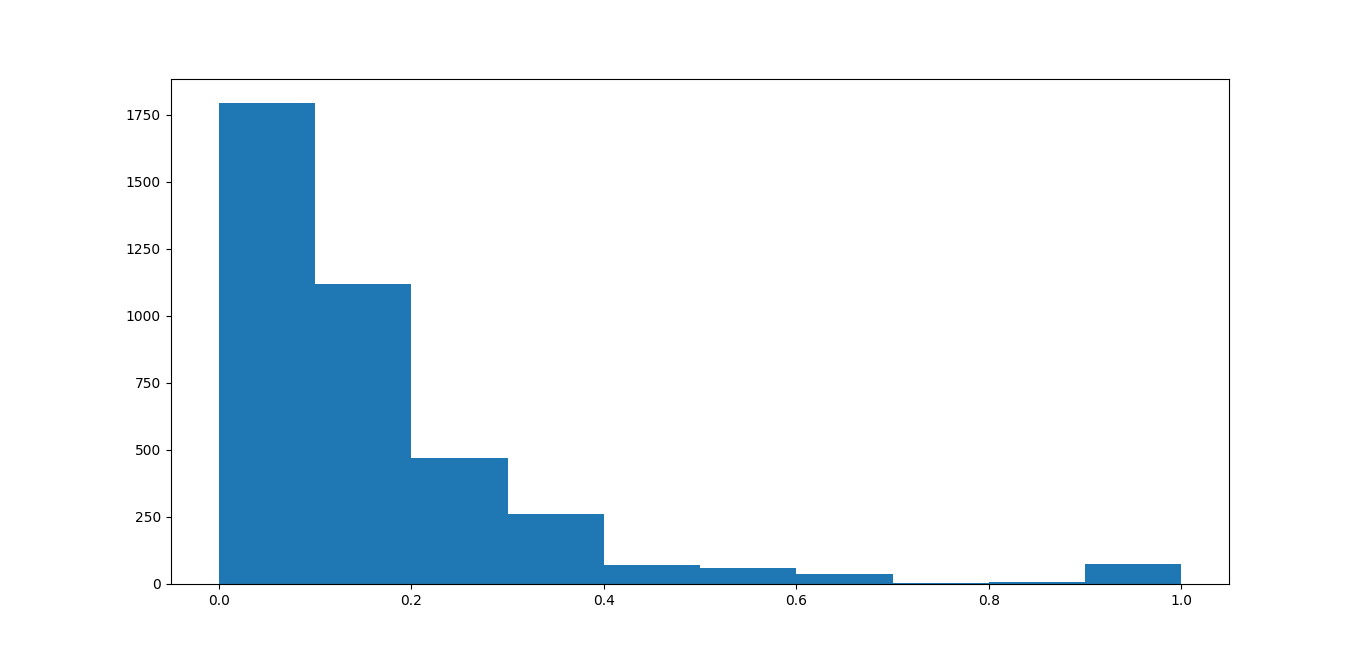
\includegraphics[width=\textwidth,height=\textheight,keepaspectratio]{clustering.png}
    \caption{Clustering graph for Part 2}
    \label{fig:part2clustering}
\end{figure}

\begin{figure}
    \centering
    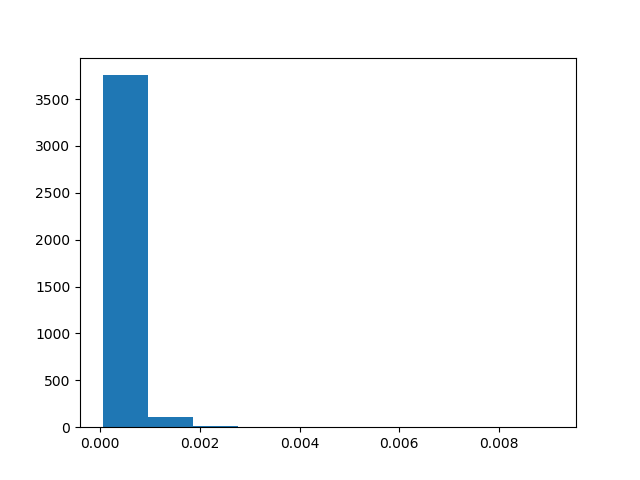
\includegraphics[width=\textwidth,height=\textheight,keepaspectratio]{page_rank.png}
    \caption{Page Rank graph for Part 2}
    \label{fig:part2pagerank}
\end{figure}

\begin{figure}
    \centering
    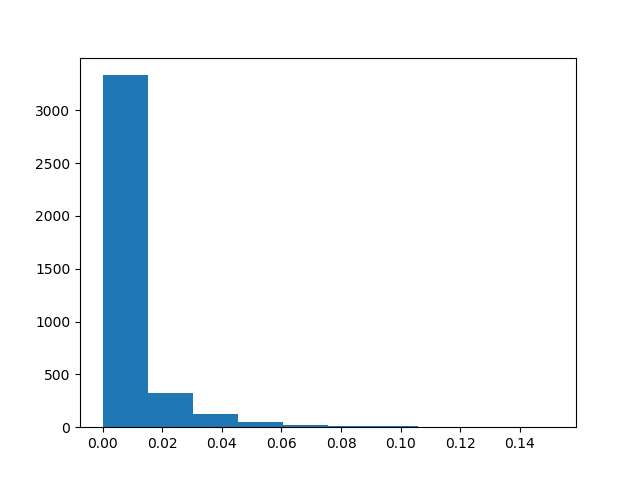
\includegraphics[width=\textwidth,height=\textheight,keepaspectratio]{eigenvector_centrality.png}
    \caption{Eigenvector Centrality for part 2}
    \label{fig:part2eignenvector}
\end{figure}

\begin{figure}
    \centering
    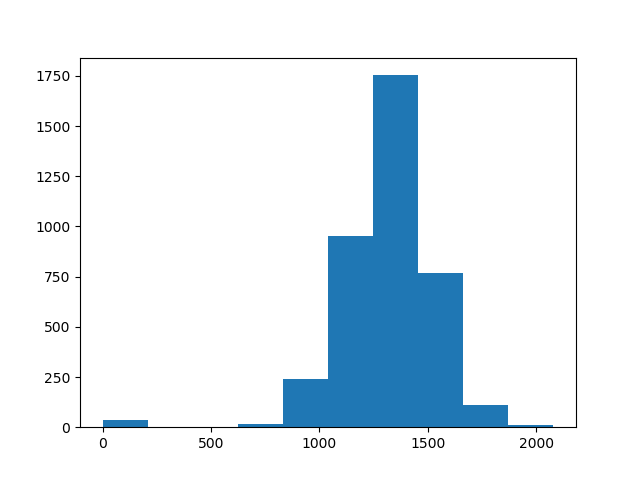
\includegraphics[width=\textwidth,height=\textheight,keepaspectratio]{harmonic_centrality.png}
    \caption{Harmonic Centrality for part 2}
    \label{fig:part2harmonic}
\end{figure}

\begin{figure}
    \centering
    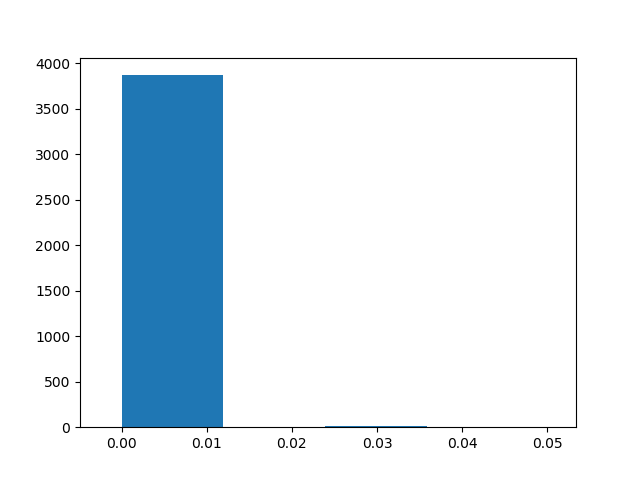
\includegraphics[width=\textwidth,height=\textheight,keepaspectratio]{betweenness_centrality.png}
    \caption{Betweenness Centrality}
    \label{fig:part2betweenness}
\end{figure}

\begin{figure}
    \centering
    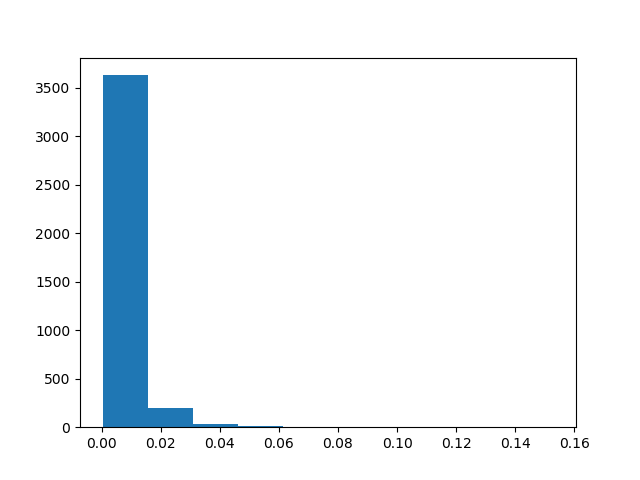
\includegraphics[width=\textwidth,height=\textheight,keepaspectratio]{degree_centrality.png}
    \caption{Degree Centrality output}
    \label{fig:part2degree}
\end{figure}

\begin{figure}
    \centering
    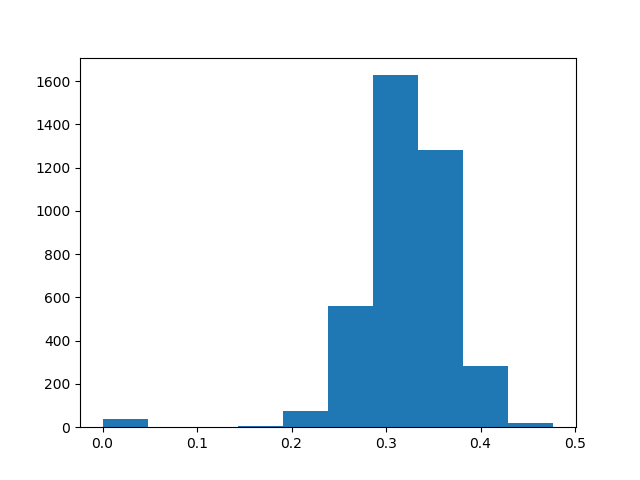
\includegraphics[width=\textwidth,height=\textheight,keepaspectratio]{closeness_centrality.png}
    \caption{CLoseness Centrality output}
    \label{fig:part2closeness}
\end{figure}

\end{document}
